%----------------------------------------------------------------------------------------
%	SECTION 1.5
%----------------------------------------------------------------------------------------

\section{Closed Sets and Limit Points.}

\begin{definition}
    A subset $A$ of a topological space  $X$ is said to be  \textbf{closed} if
    $\com{X}{A}$ is open.		
\end{definition}

\begin{example}
    \begin{enumerate}[label=(\arabic*)]
        \item Consider $[a,b] \subseteq \R$, we have that
            $\com{\R}{[a,b]}=(-\infty,a) \cup (b, \infty)$ which is open in
            $\R$. So  $[a,b]$ is closed.

        \item In  $\R \times \R$, the set  $A=\{x \times y: x,y \geq 0\}$  (i.e
            the first quadtant of the plane) is closed, for $\com{\R \times
            \R}{A}=(- \infty,0) \times \R \cup \R \times (-\infty,0)$, which is
            open in $\R \times \R$.

        \item Consider the finite complement topology $\Tc_C$ on a set  $X$. We
            have that  $\com{X}{X}=\emptyset \in \Tc$, so  $X$ is closed,
            similarly,  $\emptyset$ is also closed. Likewise, if  $A \subseteq
            X$ is a finite set, then  $\com{X}{A}$ is also finite, and hence $A$
            is also closed. Thus, we have that all the closed sets of  $\Tc_C$
            are those finite subsets of  $X$. As a consequence, this examle also
            illustrates that sets can be both closed and open.

        \item In the discrete topology  $2^X$, every open set is closed. This is
            another example where open sets are also closed sets.

        \item Consider  $[0,1] \cup (2,3)$ in the subspace topology on $\R$. We
            have that  $[0,1]$ is open  ($[0,1]=[0,1] \cup (2,3) \cap
            (-\frac{2}{3}),\frac{3}{2}$), similarly, $(2,3)$ is also open. Now
            taking  $\com{[0,1] \cup (2,3)}{(2,3)}=[0,1]$, which is open, so
            $[0,1]$ is closed in the subspace topology on  $\R$, bu the same
            reasoning, so is  $(2,3)$.
    \end{enumerate}		
\end{example} 

\begin{theorem}\label{1.6.1}
    Let $X$ be a topological space. Then:
         \begin{enumerate}[label=(\arabic*)]
             \item $\emptyset$ and  $X$ are closed.

             \item Arbitrary intersections of closed sets are closed.

             \item Finite unions of closed sets are closed.
        \end{enumerate}
\end{theorem}
\begin{proof}
    We have that $\com{X}{\emptyset}=X$ and  $\com{X}{X}=\emptyset$, both of
    which are open in  $X$, so they are also closed in  $X$. Now let
    $\{U_{\alpha}\}$ be a collection of closed sets of  $X$. We have that:
        \begin{equation*}
            \com{X}{\bigcap_{\alpha}}{U_{\alpha}}=\bigcup_{\alpha}{\com{X}{U_{\alpha}}}.
        \end{equation*}
        Similarly, for $\{U_i\}_{i=1}^{n}$, we have
        \begin{equation*}
            \com{X}{\bigcup_{i=1}^{n}}{U_{i}}=\bigcap_{i=1}^{n}{\com{X}{U_{i}}}.
        \end{equation*}
    Both of which are open in $X$. This completes the proof.
\end{proof}

\begin{definition}
    If $Y$ is a subspace of  $X$, we say that  $A$ is  \textbf{closed in $Y$} if
    $A \subseteq Y$ and  $A$ is closed in the subspace topology of  $Y$.
\end{definition}

\begin{theorem}\label{1.6.2}
    Let $Y$ be a subspace of  $X$. Then  $A$ is closed in  $Y$ if and only if
    $A$ equals the intersection of a closed set of  $X$ with  $Y$.
\end{theorem}
\begin{proof}
    Suppose that $A$ is closed in  $Y$, then  $\com{Y}{A}$ is open in  $Y$,
    hence we have that  $\com{Y}{A}=U \cap Y$ for some open set $U$ of  $X$. Now
    $\com{X}{U}$ is closed in  $X$, and with  $A \subseteq Y$, we have that
    $A=Y \cap \com{X}{U}$.

    Conversely, suppose that $A=C \cap Y$, with  $C$ closed in  $X$. Then
    $\com{X}{C}$ is open in  $X$, hence  $\com{X}{C} \cap Y$ is open in  $Y$,
    now since  $\com{X}{C} \cap Y=\com{Y}{A}$, which is open, we have that  $A$
    is closed in  $Y$.
\end{proof}

\begin{theorem}\label{1.6.3}
    Let $Y$ be a subspace of  $X$. If  $A$ is closed in  $Y$, and  $Y$ is closed
    in  $X$, then  $A$ is closed in  $X$; that is, closure is transitive.
\end{theorem}
\begin{proof}
    By theorem \ref{1.6.2}, if $A$ is closed in  $Y$, then  $A=C \cap Y$ with
    $C$ closed in  $X$, now since  $Y$ is closed in  $X$, then  $Y=D \cap X$
    with  $D$ closed in  $X$. Thus  $A=(C \cap D) \cap X$, therefore,  $A$ is
    closed in  $X$.		
\end{proof}

We now go over the concepts of the closure, and the interior of a set.

\begin{definition}
    Let $A \subseteq X$, with  $X$ a topological space. The  \textbf{interior}
    of $A$ is defined to be the union of all open sets in  $A$. The
    \textbf{closure} of $A$ is defined to be the intersection of all closed sets
    containing $A$. We denote the interior and the closure of  $A$ as  $\Int{A}$
    and  $\cl{A}$ respectively
\end{definition}

We have by the very definitions that $\Int{A} \subseteq A \subseteq \cl{A}$

\begin{lemma}\label{1.6.4}
    $\Int{A}=A$ only when  $A$ is open, and  $\cl{A}=A$ only when  $A$ is
    closed.
\end{lemma}
\begin{proof}
    Now, if $A$ is open, then it is in the union of all open sets of  $A$, hence
    $A \subseteq \Int{A}$, likewise, if  $A$ is closed, then since $\cl{A}$ is
    the intersection of all closed sets containing  $A$, we get $\cl{A}
    \subseteq A$.
\end{proof}
\begin{corollary}
    $A$ is closed and open if and only if  $\Int{A}=\cl{A}$.
\end{corollary}

\begin{theorem}\label{1.6.5}
    Let $Y$ be a subspace of  $X$, and let  $A \subseteq Y$, and let $\cl{A}$
    be the closure of $A$. Then  $\cl{A} \cap Y$ is the closure of  $A$ in
    $Y$.
\end{theorem}
\begin{proof}
    Let $\cl{A}$ be the closure of  $A$ in  $Y$. Since  $\cl{A}$ is closed in
    $X$, by theorem \ref{1.6.2},  $\cl{A} \cap Y$ is closed in  $Y$, now we
    have that $A \subseteq \cl{A} \cap Y$, and since $\cl{A}=\bigcap{U}$, then
    $\cl{A} \subseteq \cl{A} \cap Y$.

    Conversely, suppose that $\cl{A}$ is closed in  $Y$, again by theorem
    \ref{1.6.2}, we have that  $\cl{A}=C \cap Y$, where  $C$ is closed in  $X$,
    since  $A \subseteq \cl{A}$, then  $A \subseteq C$, and since  $C$ is
    closed, then  $\cl{A} \subseteq C$, thus  $\cl{A} \cap Y \subseteq
    \cl{A}$.
\end{proof}

\begin{definition}
    Let $X$ be a topological space, and let  $x \in X$. We call an open set  $U$
    of  $X$ a \textbf{neighborhood} of  $x$ if  $x \in U$.
\end{definition}

\begin{theorem}\label{1.6.6}
    If $A \subseteq X$, with  $X$ a topological space, then  $\cl{A}$ is a
    neighborhood of  $x \in X$ if and only if for every neighborhood  $U$ of
    $x$,  $A \cap U \neq \emptyset$.
\end{theorem}
\begin{proof}
    We prove the contrapositve. If $x \notin \cl{A}$, then
    $U=\com{X}{\cl{A}}$ is an open set containing  $A$, disjoint from
    $A$. Conversely, suppose there is a neighborhood $U$ of $x$, with $U$
    disjoint from  $A$, then  $\com{X}{U}$ is closed, and therefore contains the
    closure of  $A$, thus  $x \notin \cl{A}$
\end{proof}
\begin{corollary}
    $\cl{A}$ is a neighborhood of  $x$ if and only if for every basis element
    $B$ of  $X$, containing  $x$, intersects  $A$.
\end{corollary}
\begin{proof}
    This is a direct application of theorem \ref{1.6.6}, since basis elements
    are open sets.	
\end{proof}

\begin{example}
    \begin{enumerate}[label=(\arabic*)]
        \item We have the closure of $(0,1]$ in  $\R$ is the closed interval
            $[0,1]$, since every neighborhood of $0$ intersects  $(0,1]$. Now
            every point outside of  $[0,1]$ has a neighborhood disjoint from
            $[0,1]$  (take the neighborhood $(2,3)$ of  $2$).

        \item $\cl{\frac{1}{\Z^+}}=\{0\} \cup \frac{1}{\Z+}$ and $\cl{\{0\} \cup
            (1,2))}=\{0\} \cup [1,2]$.

        \item $\cl{\Q}=\R$,  $\cl{\Z^+}=\Z^+$,  $\cl{\R^+}=\R^+ \cup \{0\}$.
            This first follows from the density of $\Q$ in  $\R$. Every
            neighborhood  $n \in \Z^+$ intersects  $\Z^+$, so  $\cl{Z^+}
            \subseteq \Z^+$, and we have that the neighborhood  $(0,1)$ of  $0$ 
            intersects $\R^+$, so  $\cl{\R^+} \subseteq \R^+ \cup \{0\}$.
    \end{enumerate}		
\end{example} 

\begin{definition}
    If $A \subseteq X$, with  $X$ a topological space, and if  $x \in X$, we say
    that  $x$ is a \textbf{limit point} of  $A$ if every neighborhood of  $x$
    intersects $A$ at some distinct point. That is:  $x \in
    \cl{\com{X}{\{x\}}}$.
\end{definition}

\begin{example}
    \begin{enumerate}[label=(\arabic*)]
        \item Consider $(0,1]$, we have that  $0 \in [0,1]=\cl{(0,1]}=\cl{\com{[0,1]}{\{0\}}$, 
            so $0$ is a limit point of $(0,1]$, the same can be said for any  $x \in (0,1]$.		

        \item For $\frac{1}{\Z^+}$, $0$ is once again a limit point. 
            Let  $x \in \R$ be nonzero, and let  $[x,b)$ be the neighborhood
            of  $x$ in the lower limit topology. Then  $[x,b) \cap
            \frac{1}{\Z^+}=\emptyset$ or $\{x\}$, hence,  $0$ is the only limit
            point of  $ \frac{1}{\Z^+}$.

        \item $\cl{\{0\} \cup (1,2)}=\{0\} \cup [1,2]$ has all of its limit
            points in $[1,2]$. Likewise, every point in  $\R$ is a limit point
            of  $\Q$.  $\Z^+$ has no limit points in  $\R$, and the limit points
            of  $\R^+$ are all the points of  $\cl{\R^+}$.
    \end{enumerate}
\end{example} 

\begin{theorem}\label{1.6.7}
    Let $A \subseteq X$,  $X$ a topological space, and let  $A'$ be the set of
    all limit points in  $A$. Then  $\cl{A}=A \cup A'$.
\end{theorem}
\begin{proof}
    Let $x \in A'$, then every neighborhood of  $x$ intersects  $A$ at some
    distinct point  $x'$, by definition, so by theorem \ref{1.6.6},  $x \in
    \cl{A}$, hence $A' \subseteq \cl{A}$, so  $A \cup A' \subseteq \cl{A}$.
    Now, let $x \in \cl{A}$. If  $x \in A$, we are done. Otherwise, since every
    neighborhood of  $x$ intersects  $A$, we have that they intersect at
    distinct points, thus  $x \in A'$, therefore $\cl{A} \subseteq A \cup A' $.
\end{proof}
\begin{corollary}
    $A \subseteq X$ is closed if and only if $A' \subseteq A$.
\end{corollary}
\begin{proof}
    If $A$ is closed, then  $\cl{A}=A=A \cup A'$, thus  $A' \subseteq A$. The
    converse is obvious.		
\end{proof}

\begin{definition}
    Let $X$ be a topological space. A sequence  $\{x_n\}$ is said to
    \textbf{converge} to a point  $x \in X$ if for every neighborhood  $U$ of
    $x$, there is an  $N \in \Z^+$ such that  $x_n \in U$ for all  $n \geq N$.		
\end{definition}

\begin{example}
    Consider the following topological space on $\{a,b,c\}$ in 
    \begin{figure}[h]
        \centering
        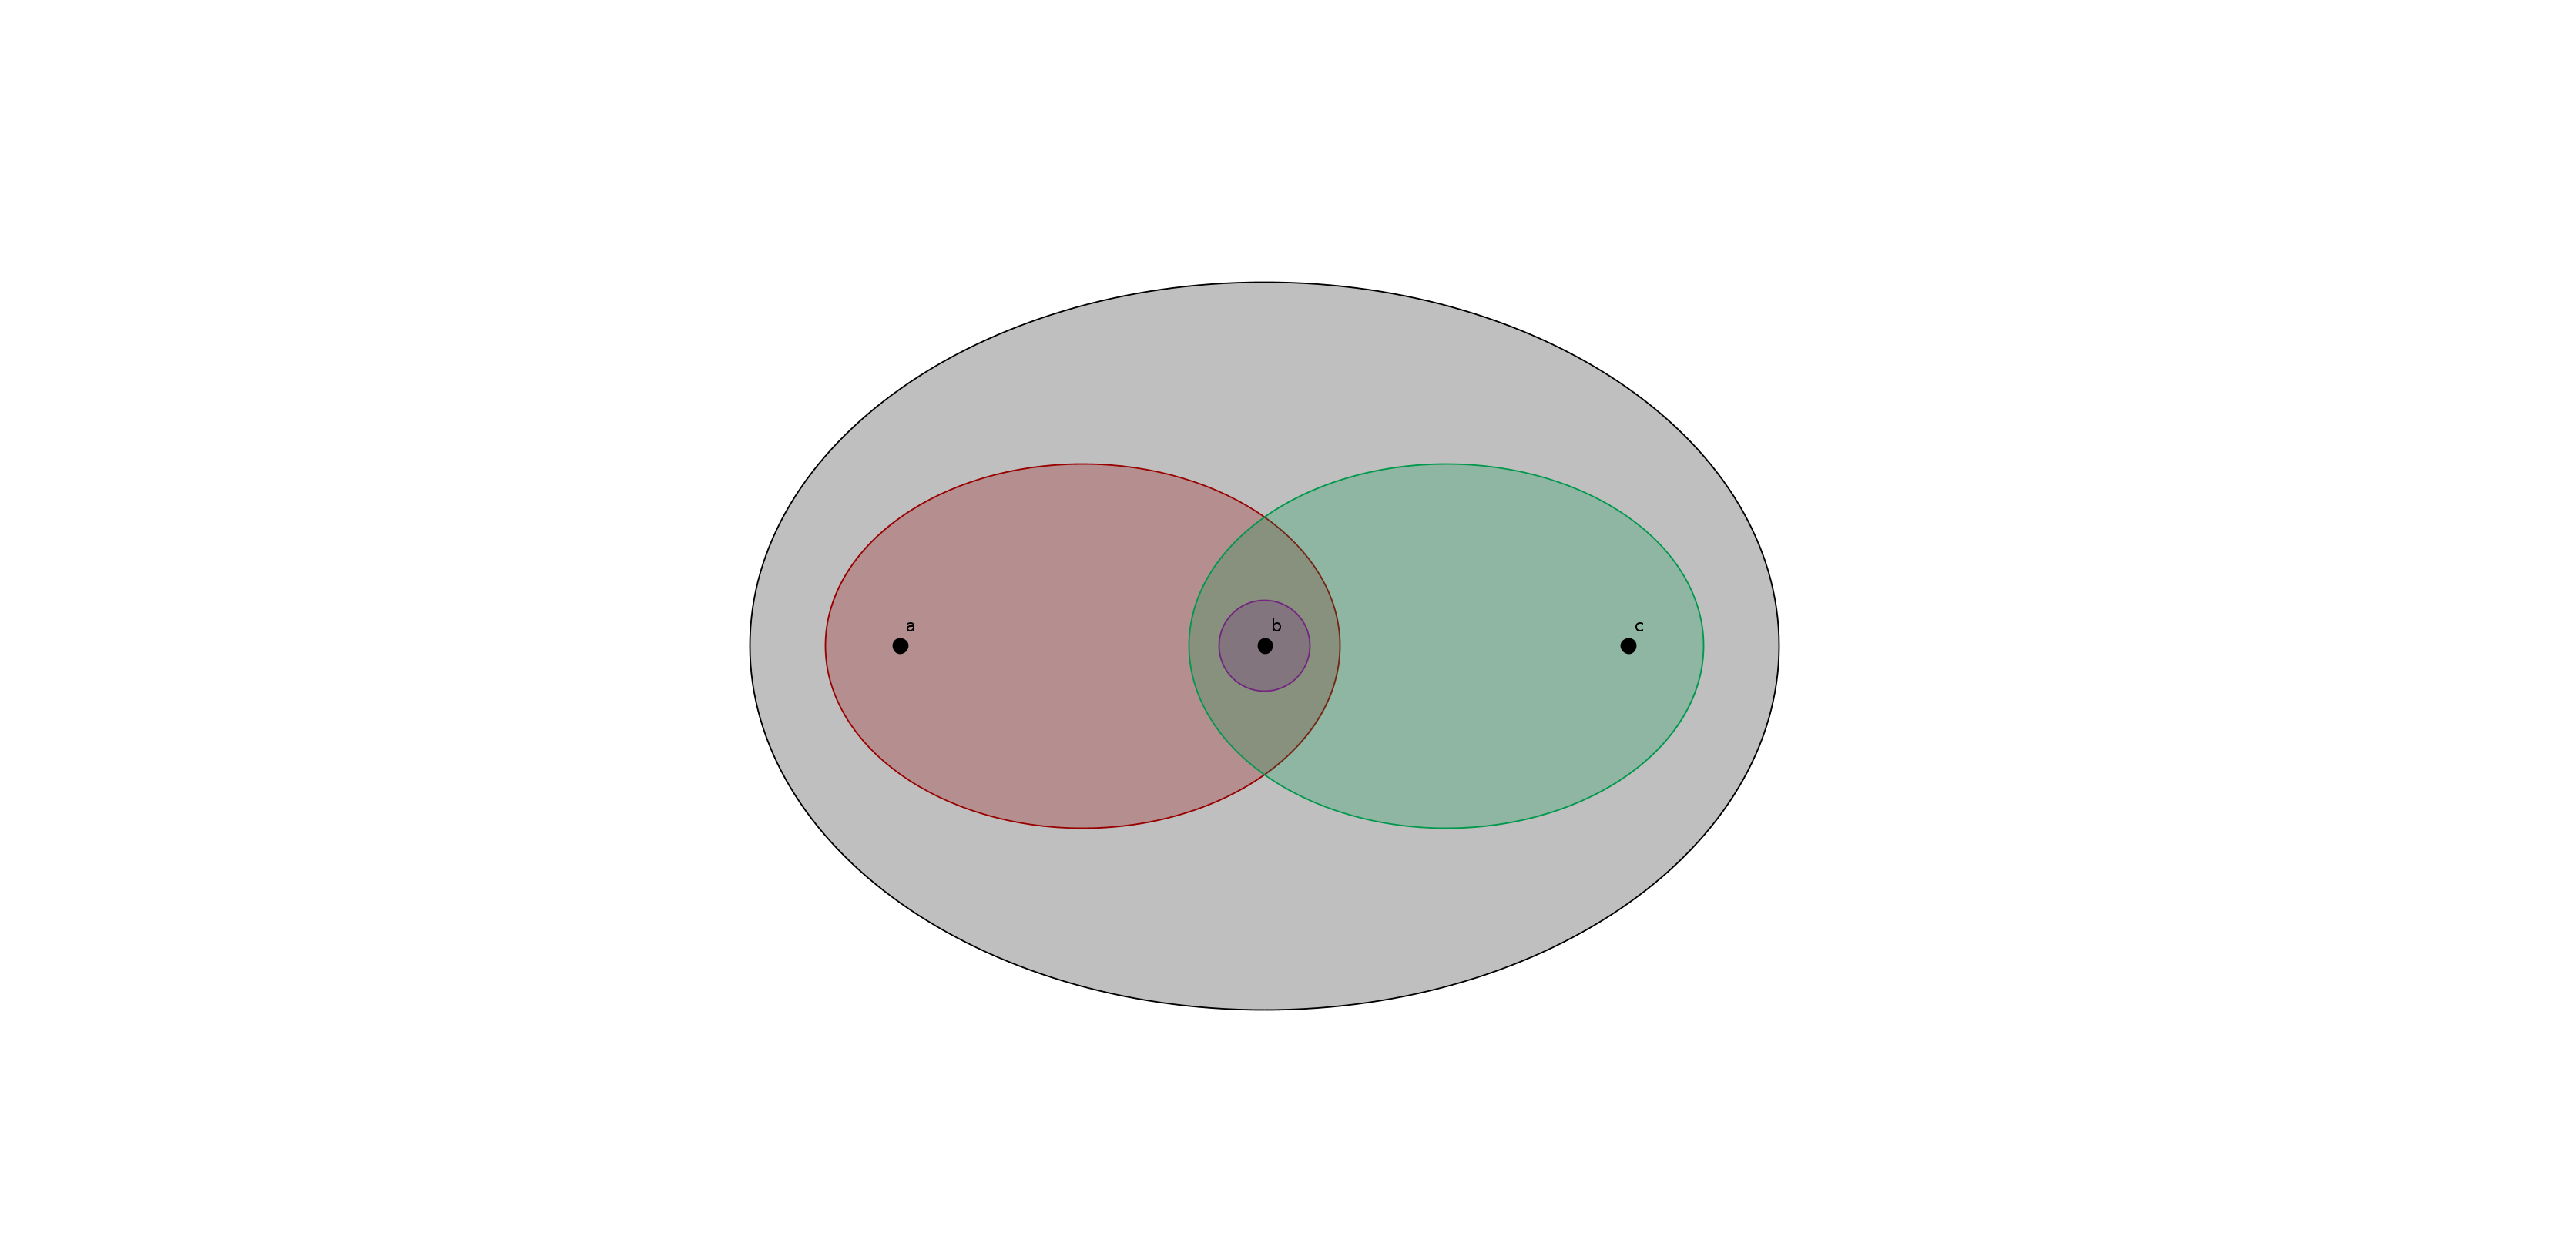
\includegraphics[scale = 0.5]{Figures/Chapter1/hausdorffSpace.png}
        \caption{A topology on $\{a,b,c\}$, which turns out to be a Hausdorff
        space.}
        \label{fig1.8}
    \end{figure}
    figure \ref{fig1.8}, and define the sequence $\{x_n\}$ by  $x_n=b$ for all
    $n \in \Z^+$. The neighborhoods of  $a$, $b$, and $c$ are
    $U_a=\{a,b\}$,  $U_b=\{b\}$, and  $U_c=\{b,c\}$. Now let $N>0$, then we see
    that for all  $n \geq N$, that  $b \in U_b,U_a,U_c$, thus  $b$
    converges to  $a$ and to  $c$, and itself,
\end{example} 

\begin{definition}
    A topological space $X$ is called a \textbf{Hausdorff space} if for each
    pair of distinct points  $ x_1$ , and $x_2$, there are neighborhoods $ U_1$
    and $U_2$ of $ x_1$ and $ x_2$ respectively such that $ U_1$ and $ u_2$ are
    disjoint.
\end{definition}

\begin{example}
    The topology of the previous example in figure \ref{1.8} is not a Hausdorff
    space.
\end{example} 

\begin{theorem}\label{1.6.8}
    Every finite point set in a Hausdorff space is closed.
\end{theorem}
\begin{proof}
    Let $X$ be a Hausdorff space, and let  $x_0 \in X$. We have that
    $\cl{\{x_0\}}=\bigcap_{\{x_0\} \in U}{U}$. Now let $x \neq x_0 \in X$.
    Since $x \in \{x_0\}$, and $X$ is Hausdorff, the inters of the neighborhoods
    of $x$ and  $ x_0$ is empty, thus $x \notin \cl{\{x_0\}}$, therefore
    $\cl{\{x_0\}}=\{x_0\}$.
\end{proof}
\begin{remark}
    We can extend this proof to finite point sets of size $n$ by induction.
\end{remark}

Now the condition that finite point sets be closed need not depend on whether or
not $X$ is a Hausdorff space. In fact, we can assume the following for some
topoltopological spaces.

\begin{axiom}[The $T_1$ Axiom]\label{axm1.6.1}
    In any topological space, every finite point set of $X$ is closed.
\end{axiom}

\begin{theorem}\label{1.6.10}
    Let $X$ be a topological space satisfying the $ T_1$ axiom, and let $A
    \subseteq X$. Then a point  $x$ is a limit point of  $A$ if and only if
    every neighborhood of  $x$ contains infinitely many points of  $A$.
\end{theorem}
\begin{proof}
    Let $U_x$ be a neighborhood of  $x$. If  $U_x$ intersects $A$ at infinitely
    many points of  $A$, then it intersects  $A$ at a point distinct from  $x$,
    thus  $x$ is a limit point of  $A$.

    Conversely suppose that  $x$ is a limit point of  $A$, and let  $U_x \cap A$
    be finite, then  $U_x \cap \com{A}{\{x\}}$. Now let  $U_x \cap
    \com{A}{\{x\}}=\{x_1, \dots x_m\}$. By the $T_1$ axiom,  $\{x_1, \dots,
    x_m\}$ is closed, so $\com{X}{\{x_1, \dots,
    x_m\}}$ is open, thus $U_x \cap \com{X}{\{x_1, \dots,
    x_m\}}$ is a neighborhood of $x$ that does not intersect  $\com{A}{\{x\}}$,
    which contradicts that  $x$ is a limit point.
\end{proof}

\begin{theorem}\label{1.6.11}
    If $X$ is a Hausdorff space, then a sequence of points of  $X$ converges to
    at most one point in  $X$.
\end{theorem}
\begin{proof}
    Let $\{x_n\}$ be a sequence of points converging to $x$, and let  $y \neq x$
    and let  $U_x$ and  $U_y$ be neighborhoods of  $x$ and  $y$ respectively.
    Then $U_x \cap U_y = \emptyset$. Now since  $\{x_n\}$ converges to  $x$, we
    have that for $N>0$, $x_n \in U_x$ whenever $n \geq N$. Then $x_n \notin
    U_y$, and so  $\{x_n\}$ cannot converge to  $y$.
\end{proof}

\begin{definition}
    Let $\{x_n\}$ be a sequence in a Hausdorff space  $X$. If  $\{x_n\}$
    converges to a point $x \in X$, we call  $x$ the \textbf{limit} of
    $\{x_n\}$ and we write  $\lim{x_n}=x$ or  $\{x_n\} \rightarrow x$.		
\end{definition}

\begin{theorem}\label{1.6.12}
    The following are true:
        \begin{enumerate}[label=(\arabic*)]
            \item Every simply oredered set under the order topology is
                Hausdorff.

            \item The product of two Hausdorff spaces is Hausdorff.

            \item The subspace of a Hausdorff space is Hausdorff.
        \end{enumerate}
\end{theorem}
\begin{proof}
    \begin{enumerate}[label=(\arabic*)]
        \item Let $X$ be an ordered set under the order topology. Take  $x,y \in
            X$ distinct, and suppose without loss of generality that $x<y$. Then
            consider the neighborhoods  $(-\infty,x]$ and  $[y,\infty)$ of  $x$
            and  $y$ respectively. Then  $(-\infty,x] \cap
            [y,\infty)=\emptyset$.

        \item Let $X$ and  $Y$ be Hausdorff, and consider  $X \times Y$ in the
            product topology. Let  $ x_1 \times y_1$ and $ x_2 \times y_2$ be
            distinct points, and let $U_{x_1}$, $U_{x_2}$, $V_{y_1}$ and
            $V_{y_2}$ be basis elements of $ x_1$, $ x_2$, $y_1$, and $y_2$
            respectively. Then they are neighborhoods of those elements
            respectively.

            Now we have that $U_{x_1} \times V_{y_1}$ and $U_{x_2} \times
            V_{y_2}$ are basis elements of $ x_1 \times y_1$ and $ x_2 \times
            y_2$, respectively, and hence neighborhoods of those elements
            respectively.Then we have $(U_{x_1} \times V_{y_1}) \cap (U_{x_2} \times
            V_{y_2})=(U_{x_1} \cap U_{x_2}) \times (V_{y_1} \cap V_{y_2}) = \emptyset
            \times \emptyset =\emptyset)$.

        \item Let $X$ be Hausdorff, and let  $Y$ be a subspace of  $X$. Let  $x_1$ 
            and $x_2$ be distinct points, and let  $U_{x_1}$ and $U_{x_2}$ be
            their neighborhoods. Since $Y$ is open in  $X$, then so are  $Y \cap
            U_{x_1}$ and $Y \cap U_{x_2}$, so they are also neighborhoods of $
            x_1$ and $ x_2$ respectively. Then $Y \cap
            U_{x_1} \cap Y \cap U_{x_2}=Y \cap (U_{x_1} \cap
            U_{x_2})=\emptyset$.
    \end{enumerate}		
\end{proof}
